% answers.tex —— 1965 年·全国卷 · 参考答案与详细解析片段
% 由 tools/generate_projects.py 依来源总账自 1965/1965_数学真题_试题.md + 1965/1965_数学真题_解析正文.md + 1965/1965_数学真题_答案要点.md 生成，勿手改（改源 MD 后重跑）


\begin{answer}
\gksolhead{1}{}

\textbf{题目}：

右面的二视图所表示的立体是什么？求出它的体积。图中底面正六边形的边长为 $a$，侧棱长为 $2a$。
\nopagebreak[4]
\begin{center}\begin{tikzpicture}[scale=0.9,>=Stealth]
  % 正视图：正六棱锥的侧棱长标为 2a
  \coordinate (V) at (2.8,3.6);
  \coordinate (L) at (0.3,0.5);
  \coordinate (R) at (5.3,0.5);
  \coordinate (M1) at (1.65,0.5);
  \coordinate (M2) at (3.95,0.5);
  \draw[thick] (L) -- (R) -- (V) -- cycle;
  \draw (V) -- (M1) (V) -- (M2);
  \draw[<->] (0.62,0.78) -- (2.63,3.28) node[midway,left] {$2a$};
  \node[below] at (2.8,0.25) {正视图};

  % 俯视图：正六边形边长为 a
  \coordinate (O) at (2.8,-1.45);
  \coordinate (H1) at (1.0,-1.45);
  \coordinate (H2) at (1.9,-0.0);
  \coordinate (H3) at (3.7,-0.0);
  \coordinate (H4) at (4.6,-1.45);
  \coordinate (H5) at (3.7,-2.9);
  \coordinate (H6) at (1.9,-2.9);
  \draw (H1) -- (H2) -- (H3) -- (H4) -- (H5) -- (H6) -- cycle;
  \draw (O) -- (H1) (O) -- (H2) (O) -- (H3)
    (O) -- (H4) (O) -- (H5) (O) -- (H6);
  \draw[<->] (1.95,-2.72) -- (3.65,-2.72) node[midway,below] {$a$};
  \node[below] at (2.8,-3.18) {俯视图};
\end{tikzpicture}
\end{center}
\nopagebreak[4]
\Needspace{4\baselineskip}
\textbf{解析}

\Needspace{5\baselineskip}
由二视图可知，该立体是正六棱锥。正六边形的边长为 $a$，因此底面面积为

\nopagebreak[4]
\[A=6\cdot\frac{\sqrt3}{4}a^2=\frac{3\sqrt3}{2}a^2.\]

\Needspace{5\baselineskip}
正六边形的外接圆半径等于边长 $a$。图中侧棱长为 $2a$，设棱锥高为 $h$，则

\nopagebreak[4]
\[h=\sqrt{(2a)^2-a^2}=\sqrt3a.\]

\Needspace{5\baselineskip}
所以体积为

\nopagebreak[4]
\[V=\frac13hA=\frac13\cdot\sqrt3a\cdot\frac{3\sqrt3}{2}a^2=\frac32a^3.\]

\gkanswer{答案：$V=\dfrac32a^3$。}

\end{answer}
\begin{answer}
\gksolhead{2}{}

\textbf{题目}：

在 $A$ 处的甲船测得乙船在北偏西 $49^\circ48'$ 的 $B$ 处，以速度 $22$ 浬/小时向正北方向行驶。甲船立即从 $A$ 处出发，以速度 $26$ 浬/小时向北偏西 $a$ 度的方向沿直线驶去，追赶乙船。问 $a$ 是多大角度时，经过一段时间，甲船能够在某处 $C$ 恰好与乙船相遇？（$\lg2.2=0.3424$，$\lg2.6=0.4150$；$\lg$ 是以 $10$ 为底的对数符号。）
\nopagebreak[4]
\begin{center}\begin{tikzpicture}[scale=0.9,>=Stealth]
  \coordinate (A) at (0,0);
  \coordinate (B) at (-1.25,1.25);
  \coordinate (C) at (-0.72,2.75);
  \draw[->] (0,-0.55) -- (0,3.45) node[above] {北};
  \draw[->] (-2.2,0) -- (2.25,0) node[right] {东};
  \node[left] at (-2.2,0) {西};
  \node[below] at (0,-0.55) {南};
  \draw[thick] (A) -- (B) -- (C);
  \draw[thick,dashed] (A) -- (C);
  \fill (A) circle (1.4pt) node[below right] {$A$};
  \fill (B) circle (1.4pt) node[left] {$B$};
  \fill (C) circle (1.4pt) node[above left] {$C$};
  \node at (-0.95,0.82) {$49^\circ48'$};
  \node at (-0.36,1.58) {$a$};
  \node[below right] at (0.15,1.6) {甲船航向};
  \node[right] at (-0.55,2.25) {乙船向北};
\end{tikzpicture}
\end{center}
\nopagebreak[4]
\begin{gktip}
原卷附有正弦、余弦对数表；本题计算直接用到的正弦对数表值为：$\lg\sin49^\circ48'=1.8830$，查表 $\lg\sin40^\circ15'=1.8104$。
\end{gktip}

\Needspace{4\baselineskip}
\textbf{解析}

\Needspace{5\baselineskip}
设甲、乙船经过 $t$ 小时在 $C$ 处相遇，则

\nopagebreak[4]
\[BC=22t,\qquad AC=26t.\]

\Needspace{5\baselineskip}
在三角形 $ABC$ 中，$\angle ABC=49^\circ48'$，$\angle BAC=49^\circ48'-a$。由正弦定理，

\nopagebreak[4]
\[\frac{26t}{\sin(180^\circ-49^\circ48')}=\frac{22t}{\sin(49^\circ48'-a)}.\]

\Needspace{5\baselineskip}
于是

\nopagebreak[4]
\[\sin(49^\circ48'-a)=\frac{22}{26}\sin49^\circ48'.\]

\Needspace{5\baselineskip}
两边取以 $10$ 为底的对数：

\nopagebreak[4]
\[\begin{aligned}
\lg\sin(49^\circ48'-a)
&=\lg2.2-\lg2.6+\lg\sin49^\circ48'\\
&=0.3424-0.4150+1.8830\\
&=1.8104.
\end{aligned}\]

\Needspace{5\baselineskip}
查正弦对数表得

\nopagebreak[4]
\[49^\circ48'-a=40^\circ15'.\]

\Needspace{5\baselineskip}
故

\nopagebreak[4]
\[a=49^\circ48'-40^\circ15'=9^\circ33'.\]

\gkanswer{答案：$a=9^\circ33'$。}

\end{answer}
\begin{answer}
\gksolhead{3}{}

\textbf{题目}：

把地球看作半径为 $R$ 的球。设 $A$、$B$ 两地的纬度相同，都是 $a$ 度，它们的经度相差 $\beta$ 度（$0^\circ<\beta\leqslant180^\circ$）。求 $A$、$B$ 两地之间的球面距离（即大圆弧长）。
\nopagebreak[4]
\begin{center}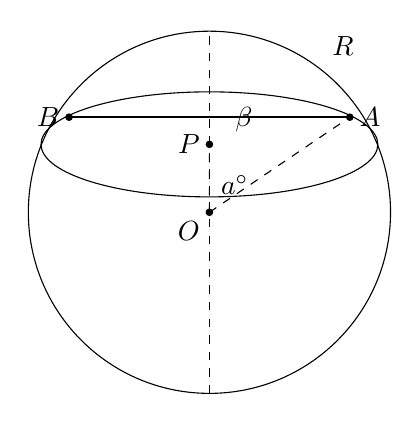
\begin{tikzpicture}[scale=1.15]
  \draw (0,0) circle (2);
  \draw[dashed] (0,-2) -- (0,2);
  \draw (0,0.75) ellipse (1.86 and 0.58);
  \coordinate (O) at (0,0);
  \coordinate (P) at (0,0.75);
  \coordinate (A) at (1.55,1.05);
  \coordinate (B) at (-1.55,1.05);
  \draw[thick] (A) -- (B);
  \draw[dashed] (O) -- (A) (O) -- (P);
  \fill (O) circle (1.2pt) node[below left] {$O$};
  \fill (P) circle (1.2pt) node[left] {$P$};
  \fill (A) circle (1.2pt) node[right] {$A$};
  \fill (B) circle (1.2pt) node[left] {$B$};
  \node at (0.38,1.02) {$\beta$};
  \node at (0.28,0.30) {$a^\circ$};
  \node[above right] at (1.25,1.62) {$R$};
\end{tikzpicture}
\end{center}
\nopagebreak[4]
\Needspace{4\baselineskip}
\textbf{解析}

\Needspace{5\baselineskip}
设 $P$ 为纬度为 $a$ 的纬度圈圆心，纬度圈半径为 $r$。在直角三角形 $OAP$ 中，

\nopagebreak[4]
\[r=R\cos a.\]

\Needspace{5\baselineskip}
设大圆弧 $AB$ 所对的圆心角为 $\theta$ 度，球面距离为 $d$，则

\nopagebreak[4]
\[d=\frac{\pi R\theta}{180}.\]

\Needspace{5\baselineskip}
由于 $\angle APB=\beta$，弦 $AB$ 在纬度圈中满足

\nopagebreak[4]
\[AB=2r\sin\frac\beta2=2R\cos a\sin\frac\beta2.\]

\Needspace{5\baselineskip}
另一方面，在等腰三角形 $OAB$ 中，

\nopagebreak[4]
\[AB=2R\sin\frac\theta2.\]

\Needspace{5\baselineskip}
故

\nopagebreak[4]
\[\sin\frac\theta2=\cos a\sin\frac\beta2.\]

\Needspace{5\baselineskip}
这里反三角函数的值按“度”计，于是

\nopagebreak[4]
\[\theta=2\arcsin\left(\cos a\sin\frac\beta2\right).\]

\Needspace{5\baselineskip}
代入球面弧长公式，得

\nopagebreak[4]
\[d=\frac{\pi R}{90}\arcsin\left(\cos a\sin\frac\beta2\right).\]

\Needspace{5\baselineskip}
若统一用弧度表示角度，则同一结论写作

\nopagebreak[4]
\[d=2R\arcsin\left(\cos\frac{a\pi}{180}\sin\frac{\beta\pi}{360}\right).\]

\gkanswer{答案：$d=\dfrac{\pi R}{90}\arcsin\left(\cos a\sin\dfrac\beta2\right)$（角按“度”计）。}

\end{answer}
\begin{answer}
\gksolhead{4}{}

\textbf{题目}：

（1） 证明 $|\sin2x|\leqslant2|\sin x|$。（$x$ 为任意值。）

（2） 已知 $n$ 为任意正整数，用数学归纳法证明 $|\sin nx|\leqslant n|\sin x|$。（$x$ 为任意值。）

\Needspace{4\baselineskip}
\textbf{解析}

\gksubpart{（1）}

\Needspace{5\baselineskip}
由二倍角公式，

\nopagebreak[4]
\[|\sin2x|=|2\sin x\cos x|=2|\sin x|\,|\cos x|\leqslant2|\sin x|.\]

\gksubpart{（2）}

当 $n=1$ 时，$|\sin x|\leqslant|\sin x|$ 成立。

\Needspace{5\baselineskip}
假设当 $n=k$ 时有

\nopagebreak[4]
\[|\sin kx|\leqslant k|\sin x|.\]

\Needspace{5\baselineskip}
则由和角公式及绝对值不等式，

\nopagebreak[4]
\[\begin{aligned}
|\sin(k+1)x|
&=|\sin kx\cos x+\cos kx\sin x|\\
&\leqslant|\sin kx|\,|\cos x|+|\cos kx|\,|\sin x|\\
&\leqslant k|\sin x|+|\sin x|\\
&=(k+1)|\sin x|.
\end{aligned}\]

因此由数学归纳法，对一切正整数 $n$ 都有 $|\sin nx|\leqslant n|\sin x|$。

\gkanswer{答案（1）：见解析版}

\gkanswer{答案（2）：见解析版}

\end{answer}
\begin{answer}
\gksolhead{5}{}

\textbf{题目}：

\Needspace{5\baselineskip}
已知一点 $P$ 的坐标是 $(4,-2)$，直线 $l$ 的方程是 $y-x+5=0$，曲线 $C$ 的方程是

\nopagebreak[4]
\[\frac{(x+1)^2}{2}+\frac{(y-1)^2}{4}=1.\]

求经过 $P$ 点而与 $l$ 垂直的直线和曲线 $C$ 的交点坐标，并画出此题的略图。
\nopagebreak[4]
\begin{center}\begin{tikzpicture}[scale=0.9,>=Stealth]
  \draw[->] (-3.0,0) -- (3.8,0) node[right] {$x$};
  \draw[->] (0,-3.0) -- (0,3.3) node[above] {$y$};
  \draw (0,0) ellipse (1.45 and 2.15);
  \draw[thick] (-2.2,2.2) -- (3.2,-3.2);
  \coordinate (I1) at (0.48,1.72);
  \coordinate (I2) at (-1.05,3.0);
  \fill (I1) circle (1.3pt) node[right] {$\left(\frac13,\frac53\right)$};
  \fill (I2) circle (1.3pt) node[above left] {$(-1,3)$};
  \fill (2.6,-2.6) circle (1.3pt) node[below right] {$P(4,-2)$};
  \node[below left] at (0,0) {$O$};
  \node at (1.75,1.35) {$C$};
\end{tikzpicture}
\end{center}
\nopagebreak[4]
\Needspace{4\baselineskip}
\textbf{解析}

\Needspace{5\baselineskip}
直线 $l$ 的斜率为 $1$，所以过 $P(4,-2)$ 且垂直于 $l$ 的直线斜率为 $-1$，其方程为

\nopagebreak[4]
\[y+2=-(x-4),\qquad x+y-2=0.\]

\Needspace{5\baselineskip}
由 $y=-x+2$ 代入椭圆方程，得

\nopagebreak[4]
\[\frac{(x+1)^2}{2}+\frac{(-x+1)^2}{4}=1,\]

\Needspace{5\baselineskip}
即

\nopagebreak[4]
\[3x^2+2x-1=0=(3x-1)(x+1).\]

\Needspace{5\baselineskip}
因此

\nopagebreak[4]
\[x=\frac13\quad\text{\text{或}}\quad x=-1.\]

\Needspace{5\baselineskip}
代回 $y=-x+2$，得到两个交点

\nopagebreak[4]
\[\left(\frac13,\frac53\right),\qquad(-1,3).\]

\gkanswer{答案：垂线为 $x+y-2=0$；交点为 $\left(\dfrac13,\dfrac53\right)$、$(-1,3)$。}

\end{answer}
\begin{answer}
\gksolhead{6}{}

\textbf{题目}：

当 $p$ 是什么实数时，方程 $x^2+px-3=0$ 与方程 $x^2-4x-(p-1)=0$ 有一个公共根？并求出这个公共根。

\Needspace{4\baselineskip}
\textbf{解析}

\Needspace{5\baselineskip}
设两方程的公共根为 $x$。将第二式改写为

\nopagebreak[4]
\[p=x^2-4x+1.\]

\Needspace{5\baselineskip}
代入第一方程 $x^2+px-3=0$，得

\nopagebreak[4]
\[x^2+x(x^2-4x+1)-3=0,\]

\Needspace{5\baselineskip}
即

\nopagebreak[4]
\[x^3-3x^2+x-3=0=(x-3)(x^2+1).\]

\Needspace{5\baselineskip}
由于公共根及 $p$ 都要求为实数，$x^2+1=0$ 不产生实根，所以 $x=3$。代入第一方程得

\nopagebreak[4]
\[9+3p-3=0,\]

故 $p=-2$。

\begin{gktip}
\textbf{源卷核验注}：固定答案页在代入 $x=3$ 的中间行印作“$q+3p-3=0$”；结合前式与原方程，此处应为 $9+3p-3=0$，本解析按可复核的正确式书写。答案页另一种根式枚举中还有局部符号排版疑点，但不影响实根结论 $p=-2$、$x=3$。
\end{gktip}

\gkanswer{答案：$p=-2$，公共根为 $3$。}

\end{answer}
\begin{answer}
\gksolhead{7}{}

\textbf{题目}：

已给抛物线 $y^2=2x$。

\Needspace{5\baselineskip}
（1） 在抛物线上任取两点 $P_1(x_1,y_1)$、$P_2(x_2,y_2)$。经过线段 $P_1P_2$ 的中点作直线平行于抛物线的轴，和抛物线交于点 $P_3$。证明

\nopagebreak[4]
\[\triangle P_1P_2P_3\text{ \text{的面积}}=\frac1{16}|y_1-y_2|^3.\]

（2） 经过线段 $P_1P_3$ 和 $P_2P_3$ 的中点，分别作直线平行于抛物线的轴，和抛物线依次交于 $Q_1$、$Q_2$。试将 $\triangle P_1P_3Q_1$ 与 $\triangle P_2P_3Q_2$ 的面积的和用 $y_1$、$y_2$ 表示出来。

（3） 仿照（2），又可以作出四个更小的三角形。照这样继续下去，可以作出一系列的三角形。由此设法求出线段 $P_1P_2$ 与抛物线所围成的图形的面积。
\nopagebreak[4]
\begin{center}\begin{tikzpicture}[scale=0.9,>=Stealth]
  \draw[->] (-0.35,0) -- (4.5,0) node[right] {$x$};
  \draw[->] (0,-2.35) -- (0,2.35) node[above] {$y$};
  \draw[domain=-2.1:2.1,smooth,variable=\t,thick]
    plot ({0.5*\t*\t},{\t});
  \coordinate (P1) at (3.2,1.7);
  \coordinate (P2) at (2.6,-1.55);
  \coordinate (P3) at (0.22,0.08);
  \coordinate (Q1) at (0.92,0.89);
  \coordinate (Q2) at (0.72,-0.74);
  \draw[thick] (P1) -- (P2) -- (P3) -- cycle;
  \draw[thick] (P1) -- (Q1) -- (P3);
  \draw[thick] (P2) -- (Q2) -- (P3);
  \draw[dashed] (P3) -- (Q1) (P3) -- (Q2);
  \fill (P1) circle (1.3pt) node[above right] {$P_1$};
  \fill (P2) circle (1.3pt) node[below right] {$P_2$};
  \fill (P3) circle (1.3pt) node[left] {$P_3$};
  \fill (Q1) circle (1.3pt) node[above right] {$Q_1$};
  \fill (Q2) circle (1.3pt) node[below right] {$Q_2$};
\end{tikzpicture}
\end{center}
\nopagebreak[4]
\Needspace{0.25\textheight}
\textbf{附加题}

\Needspace{5\baselineskip}
（1） 已知 $a$、$b$、$c$ 为实数，证明 $a$、$b$、$c$ 都为正数的充要条件是：

\nopagebreak[4]
\[a+b+c>0,\qquad ab+bc+ca>0,\qquad abc>0.\]

\Needspace{5\baselineskip}
（2） 已知方程

\nopagebreak[4]
\[x^3+px^2+qx+r=0\]

\Needspace{5\baselineskip}
的三个根 $\alpha$、$\beta$、$\gamma$ 都是实数，证明 $\alpha$、$\beta$、$\gamma$ 是一个三角形的三个边长的充要条件是

\nopagebreak[4]
\[p<0,\qquad q>0,\qquad r<0,\qquad p^3>4pq-8r.\]

\Needspace{4\baselineskip}
\textbf{解析}

\Needspace{5\baselineskip}
抛物线 $y^2=2x$ 可写为 $x=\dfrac{y^2}{2}$。设 $P_3$ 的纵坐标为 $y_3$。由于过 $P_1P_2$ 中点作的是平行于抛物线轴的直线，

\nopagebreak[4]
\[y_3=\frac{y_1+y_2}{2}.\]

\gksubpart{（1）}

\Needspace{5\baselineskip}
三角形面积等于行列式绝对值的一半：

\nopagebreak[4]
\[\triangle P_1P_2P_3=\frac12\left|\begin{vmatrix}1&x_1&y_1\\1&x_2&y_2\\1&x_3&y_3\end{vmatrix}\right|.\]

\Needspace{5\baselineskip}
代入 $x_i=\dfrac{y_i^2}{2}$ 及 $y_3=\dfrac{y_1+y_2}{2}$ 化简，得

\nopagebreak[4]
\[\triangle P_1P_2P_3=\frac1{16}|y_1-y_2|^3.\]

\gksubpart{（2）}

\Needspace{5\baselineskip}
对 $P_1P_3$ 和 $P_2P_3$ 分别使用（1）的结论。因为

\nopagebreak[4]
\[|y_1-y_3|=|y_3-y_2|=\frac12|y_1-y_2|,\]

\Needspace{5\baselineskip}
所以两个小三角形的面积各为

\nopagebreak[4]
\[\frac1{16}\left(\frac12|y_1-y_2|\right)^3=\frac18\cdot\frac1{16}|y_1-y_2|^3.\]

\Needspace{5\baselineskip}
它们的面积和为

\nopagebreak[4]
\[A_2=\frac14A_1=\frac1{64}|y_1-y_2|^3,\]

其中 $A_1=\dfrac1{16}|y_1-y_2|^3$。

\gksubpart{（3）}

\Needspace{5\baselineskip}
继续作中点三角形时，每一步新产生的三角形面积和都是上一步的 $\dfrac14$。因此所围图形的面积为等比级数

\nopagebreak[4]
\[\begin{aligned}
A&=A_1+A_2+A_3+\cdots\\
&=A_1\left(1+\frac14+\frac1{4^2}+\cdots\right)\\
&=\frac{A_1}{1-\frac14}=\frac43\cdot\frac1{16}|y_1-y_2|^3\\
&=\frac1{12}|y_1-y_2|^3.
\end{aligned}\]

\begin{gktip}
\textbf{源卷核验注}：固定答案页 q7 的中间行将 $|y_1-y_3|=|y_3-y_2|$ 的比例印作 $\frac1{12}|y_1-y_2|$，但随后使用 $1/2^3$ 且最终答案均对应 $\frac12|y_1-y_2|$；本解析按中点定义和后续计算采用可复核的 $\frac12$。
\end{gktip}

\gksubpart{附加题（1）}

设 $a,b,c$ 为实数。必要性显然：若三者均为正数，则 $a+b+c$、$ab+bc+ca$、$abc$ 均为正。

\Needspace{5\baselineskip}
反之，若 $abc>0$ 而三者不全为正，则恰有两个为负。设 $a=-u$、$b=-v$、$c=w$，其中 $u,v,w>0$。由题设

\nopagebreak[4]
\[w>u+v,\qquad uv>w(u+v).\]

两式合起来给出 $uv>(u+v)^2$，这与 $(u+v)^2\geqslant4uv$ 矛盾。因此 $a,b,c$ 必全为正数。

\gksubpart{附加题（2）}

\Needspace{5\baselineskip}
设三根为 $\alpha$、$\beta$、$\gamma$。由韦达定理，

\nopagebreak[4]
\[\alpha+\beta+\gamma=-p,\qquad \alpha\beta+\beta\gamma+\gamma\alpha=q,\qquad \alpha\beta\gamma=-r.\]

\Needspace{5\baselineskip}
三根成为三角形的三边，当且仅当

\nopagebreak[4]
\[u=\beta+\gamma-\alpha>0,\quad v=\gamma+\alpha-\beta>0,\quad w=\alpha+\beta-\gamma>0.\]

\Needspace{5\baselineskip}
计算这三个量的基本对称式：

\nopagebreak[4]
\[u+v+w=-p,\]

\nopagebreak[4]
\[uv+vw+wu=4q-p^2,\]

\nopagebreak[4]
\[uvw=p^3-4pq+8r.\]

\Needspace{5\baselineskip}
若 $\alpha,\beta,\gamma$ 是三角形三边，则它们本身为正数，所以 $p<0$、$q>0$、$r<0$；同时 $u,v,w>0$，从而 $uvw>0$，即

\nopagebreak[4]
\[p^3>4pq-8r.\]

\Needspace{5\baselineskip}
反过来，若

\nopagebreak[4]
\[p<0,\qquad q>0,\qquad r<0,\qquad p^3>4pq-8r,\]
\Needspace{5\baselineskip}
则 $-p>0$ 且 $uvw>0$。又因 $r<0$，有 $-8r>0$，故

\nopagebreak[4]
\[p^3>4pq-8r>4pq.\]

由于 $p<0$，除以 $p$ 时不等号变向，得到 $p^2<4q$，即 $uv+vw+wu>0$。由附加题（1）应用于 $u,v,w$，可知 $u,v,w$ 全为正数，正好说明 $\alpha,\beta,\gamma$ 满足三角形三边不等式。充要性得证。

\gkanswer{答案（1）：$\dfrac1{16}|y_1-y_2|^3$。}

\gkanswer{答案（2）：面积和为 $\dfrac1{64}|y_1-y_2|^3$。}

\gkanswer{答案（3）：所围图形面积为 $\dfrac1{12}|y_1-y_2|^3$。}

\end{answer}